\documentclass[11pt,a4paper,ngerman]{article}
\usepackage[bottom=2.5cm,top=2.5cm]{geometry} 
\usepackage{babel}
\usepackage[utf8]{inputenc} 
\usepackage[T1]{fontenc} 
\usepackage{ae} 
\usepackage{amssymb} 
\usepackage{amsmath} 
\usepackage{graphicx}
\usepackage{fancyhdr}
\usepackage{fancyref}
\usepackage{listings}
\usepackage{xcolor}
\usepackage{paralist}
\usepackage{subfigure}

%\usepackage[pdftex, bookmarks=false, pdfstartview={FitH}, linkbordercolor=white]{hyperref}
\usepackage{fancyhdr}
\pagestyle{fancy}
\fancyhead[C]{CoMa II}
\fancyhead[L]{Übung Nr. 5}
\fancyhead[R]{SoSe 2012}
\fancyfoot{}
\fancyfoot[L]{}
\fancyfoot[C]{\thepage / \pageref{LastPage}}
\renewcommand{\footrulewidth}{0.5pt}
\renewcommand{\headrulewidth}{0.5pt}
\setlength{\parindent}{0pt} 
\setlength{\headheight}{0pt}

\author{Tutor: Sebastian Scherer}
\date{}
\title{Max Wisniewski , Alexander Steen}

\begin{document}

\lstset{language=Pascal, basicstyle=\ttfamily\fontsize{10pt}{10pt}\selectfont\upshape, commentstyle=\rmfamily\itshape\small, keywordstyle=\rmfamily\bfseries, breaklines=true, frame=single, xleftmargin=3mm, xrightmargin=3mm, tabsize=2}

\maketitle
\thispagestyle{fancy}


%% ------------------------------------------------------
%%                     AUFGABE 1
%% ------------------------------------------------------

\section*{Aufgabe 1}
Das folgende matlab-Programm rechnet für $k= 1,2,6$ die jeweiligen Newton-Cotes-Formeln aus. Für andere Eingaben von $k$ wird das Program mit einem Fehler terminieren. Der Aufwand ist jeweils auf die Berechnung des Programms bezogen, welche Funktionsauswertungen nicht mehrfach benutzt und darum etwas ineffizienter ist, als es sein könnte. Allerdings wurde in der Aufgabe nichts von Effizienz gesagt, also ist das ja kein Problem.

\begin{lstlisting}[language=matlab]
function [S,A] = sumnc(ab,f,k,n)
% ab Integrationsintervall
% f zu intigrierende Funktion
% k regel der newton-cotes-formel
% n anzahl der teilintervalle

% Bezeichnungen ab hier wie im Skript
% h ist der Abstand zwischen den Stellen
h = (ab(2) - ab(1))/n;
% z sind die Stuetzstellen
z = ab(1) + (1:n).*h;

% Gewichte jeweils aus dem Skript entnommen,
% sowie Berechnungsvorgehen

if (k == 1) %% Trapez
   x = @(k) z(k);
   S = h/2 * (f(ab(1)) + f(ab(2)));
   A = 2; % Bereits 2 Auswertungen
   for k = 2:(n),
      S = S + h*f(x(k)); % Siehe Skript
      A = A+1; % Eine Berechnung mehr
   end
   return % Aufwand n+1
elseif (k == 2) %% Simpson
   % (Algorithmisches) Vorgehen analog zu Trapez
   x = @(k,j) z(k/2) + j*h/2;
   S = 0;
   A = 0;
   for k = 1:(n),
      S = S + h/6 * (f(x(2*k,0)) + 4*f(x(2*k,1)) + f(x(2*k,2)));
      A = A + 3;
   end
   return % Aufwand 3n
elseif (k == 6) %% Weddle-Regel
   x = @(k,j) z(k/6) + j*h/6;
   S = 0; A = 0;
   for k = 1:n,
      S = S + h/840 * (41*f(x(6*k,0)) + 216*f(x(6*k,1)) + 27*f(x(6*k,2)) + 272*f(x(6*k,3)) + 27*f(x(6*k,4)) + 216*f(x(6*k,5)) + 41*f(x(6*k,6)));
      A = A + 6;
   end
   return %Aufwand 6n
end
\end{lstlisting}

\begin{description}
\item[a)] 
Die Auswertungen wurden sowohl bei a) als auch bei b) mit folgendem Code gemacht (natürlich bei beiden Teilaufgaben mit verschiedenen Funktionen f und Grenzen ab)
\begin{lstlisting}[language=matlab]
>> for k = 1:50,                         
erg(k) = sumnc(ab,f,1,6*k);           
end
>> for k = 1:50,              
erg2(k) = sumnc(ab,f,2,6*k);
end
>> for k = 1:50,               
erg3(k) = sumnc(ab,f,6,6*k);
end
\end{lstlisting}

Und dann mit diesem Code geplottet (Achsenbenennung weggelassen):

\begin{lstlisting}[language=matlab]
h=loglog(6:6:6*50,abs(2-erg)) 
h2=loglog(6:6:6*50,abs(2-erg2)) 
h3=loglog(6:6:6*50,abs(2-erg3)) 
\end{lstlisting}

Dies kann man machen, da das exakte Integral $\int_0^{\pi} \sin(x) \, dx = 2$.

\begin{figure}[ht]
\centering
\subfigure[Fehler über Teilintervalle]{
	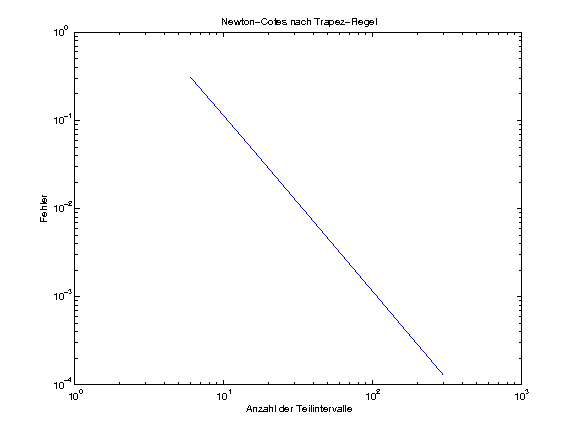
\includegraphics[scale=0.33]{diagrammeA/trapez.png}
}
\subfigure[Aufwand über Fehler]{
	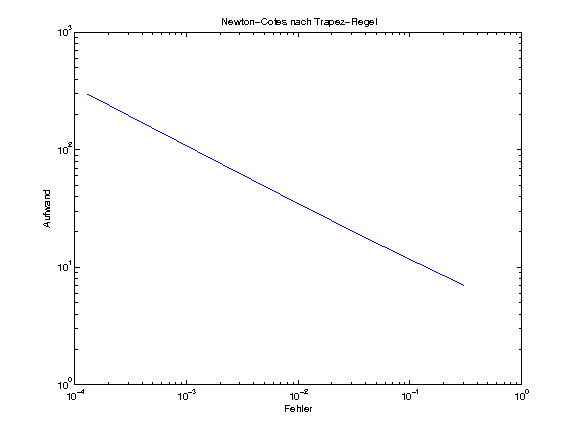
\includegraphics[scale=0.33]{diagrammeA/trapezauf.png}
}
\caption{Newton-Cotes-Formel nach Trapez-Regel}
\end{figure}

\begin{figure}[ht]
\centering
\subfigure[Fehler über Teilintervalle]{
	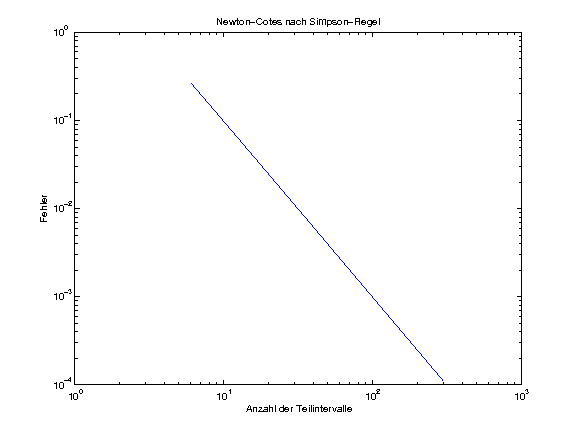
\includegraphics[scale=0.33]{diagrammeA/simpson.png}
}
\subfigure[Aufwand über Fehler]{
	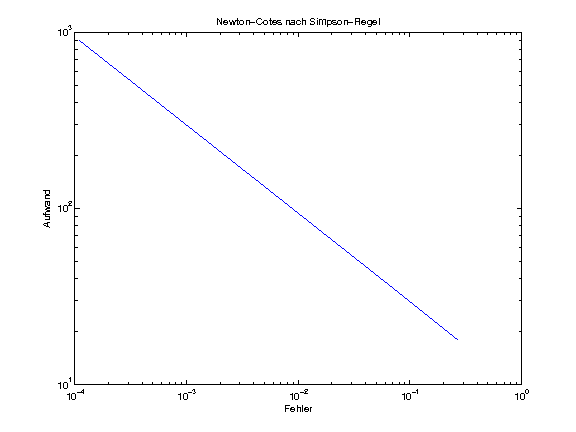
\includegraphics[scale=0.33]{diagrammeA/simpsonauf.png}
}
\caption{Newton-Cotes-Formel nach Simpson-Regel}
\end{figure}

\begin{figure}[ht]
\centering
\subfigure[Fehler über Teilintervalle]{
	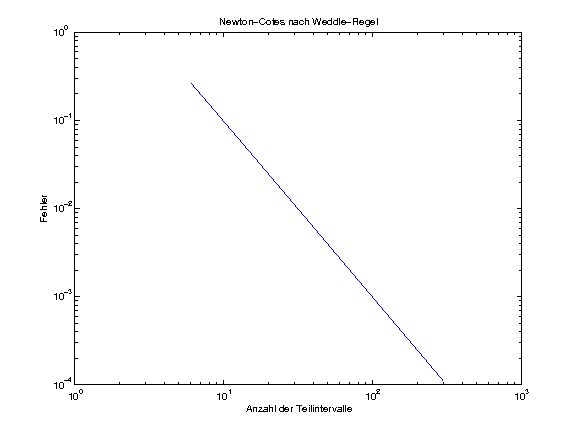
\includegraphics[scale=0.33]{diagrammeA/weddle.png}
}
\subfigure[Aufwand über Fehler]{
	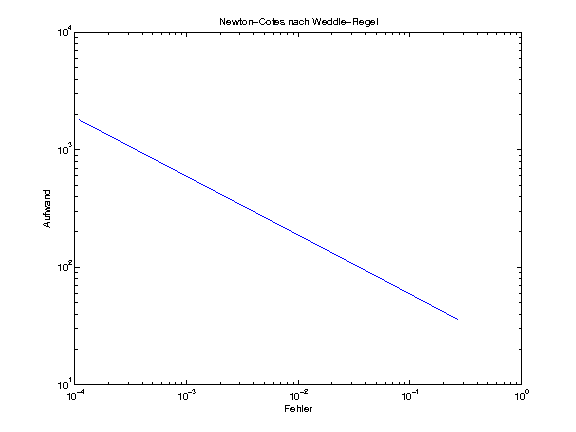
\includegraphics[scale=0.33]{diagrammeA/weddleauf.png}
}
\caption{Newton-Cotes-Formel nach Weddle-Regel}
\end{figure}

\newpage

\item[b)] Berechnung analog zu a). Hier ist der exakte Wert des Integrals $\int_0^1 \left( \sqrt(x) + \sin(21\pi x)\right) \, dx = \frac{2}{21} \left(7 + \frac{1}{\pi} \right)$. Dies haben wir so in matlab eingegeben und als Vergleichswert benutzt.

\begin{figure}[ht]
\centering
\subfigure[Fehler über Teilintervalle]{
	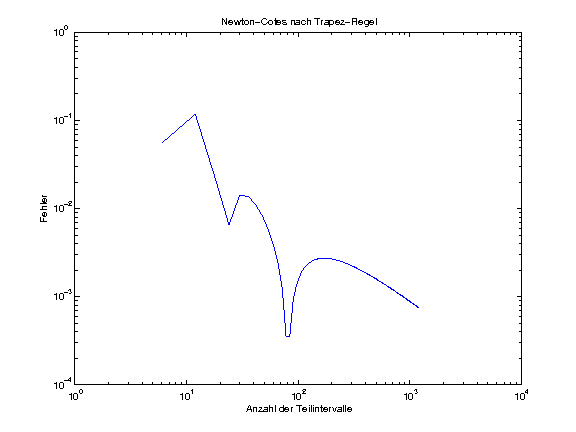
\includegraphics[scale=0.33]{diagrammeB/trapez.png}
}
\subfigure[Aufwand über Fehler]{
	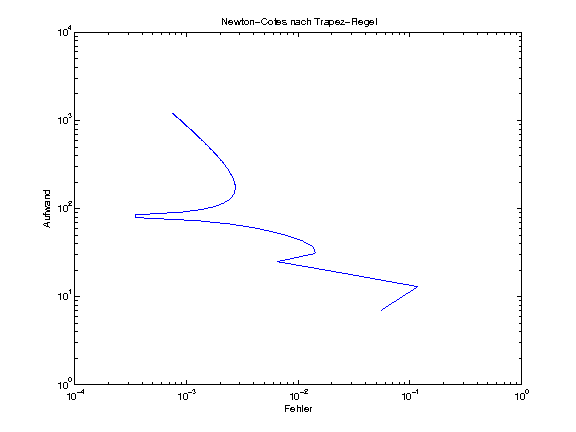
\includegraphics[scale=0.33]{diagrammeB/trapezauf.png}
}
\caption{Newton-Cotes-Formel nach Trapez-Regel}
\end{figure}

\begin{figure}[ht]
\centering
\subfigure[Fehler über Teilintervalle]{
	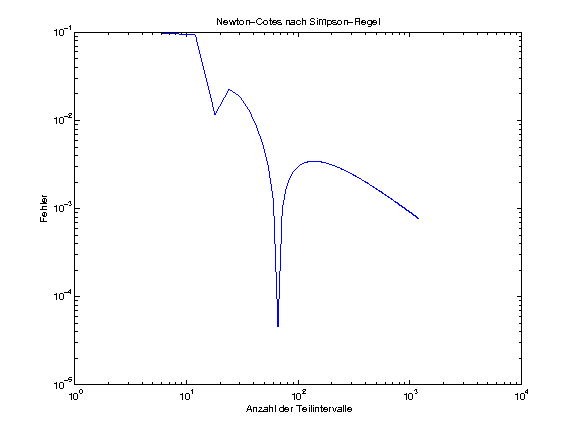
\includegraphics[scale=0.33]{diagrammeB/simpson.png}
}
\subfigure[Aufwand über Fehler]{
	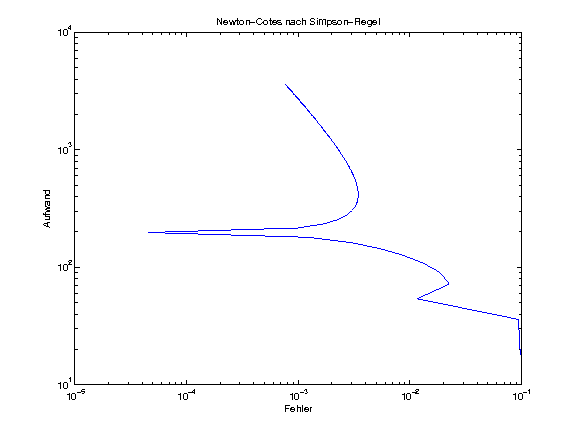
\includegraphics[scale=0.33]{diagrammeB/simpsonauf.png}
}
\caption{Newton-Cotes-Formel nach Simpson-Regel}
\end{figure}

\begin{figure}[ht]
\centering
\subfigure[Fehler über Teilintervalle]{
	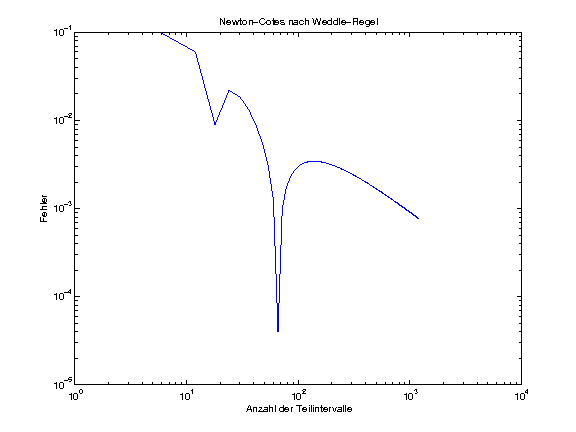
\includegraphics[scale=0.33]{diagrammeB/weddle.png}
}
\subfigure[Aufwand über Fehler]{
	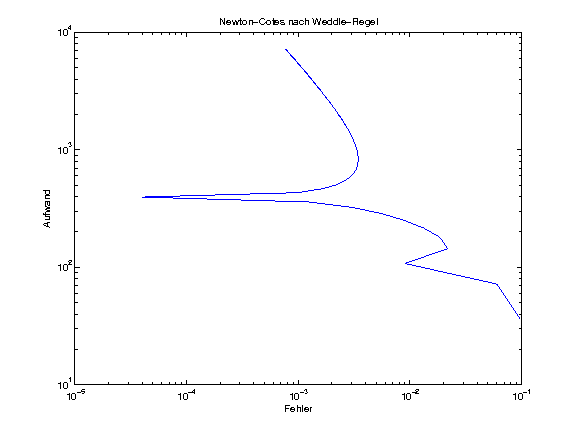
\includegraphics[scale=0.33]{diagrammeB/weddleauf.png}
}
\caption{Newton-Cotes-Formel nach Weddle-Regel}
\end{figure}
\newpage
Schaut man sich die Integrale an, so stellt man fest, dass die erste Funktion eine glatten Bogen beschreibt und die zweite Funktion extrem springt, also viele starke Variationen enthält.

\begin{figure}[ht]
\centering
\subfigure[$\int_0^{\pi} \sin(x) \, dx$]{
	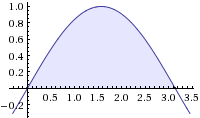
\includegraphics[scale=0.5]{sin.png}
}
\subfigure[$\int_0^1 \left( \sqrt(x) + \sin(21\pi x)\right) \, dx$]{
	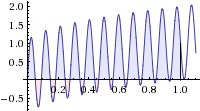
\includegraphics[scale=0.5]{snd.png}
}
\caption{Graphische Darstellung der beiden Integrale (von: Wolframalpha.com)}
\end{figure}
\end{description}
Der lineare Verlauf (auf der log-Skala) der Fehler über die Teilintervalle zeigt ein akzeptables Verhältnis und ist bei allen drei Formeln (nahezu) gleich. Dadurch, dass die Variationen des ersten Integrals sehr begrenzt sind, haben wir kleine Fehler. Auch der Aufwand steht in einem guten Verhältnis zum Fehler und ist bei allen drei Verfahren (bis auf die Konstante) gleich.
\\
\\
Bei der zweiten Integration fallen die starken Variationen bzw. die geringe Glattheit eine extreme Rolle bei den entstehenden Fehlern. Je nach Anzahl der Teilintervalle variiert die Genauigkeit der numerischen Integration sehr stark, erreicht aber bei allen drei Formeln bei ungefähr $10^2$ Teilintervallen ein relativ gutes Ergebnis. Dabei ist aber auch zu erkennen, dass der Aufwand nicht sehr gleichmäßig auf die Fehler aufgeteilt ist. Hier ähneln sich die drei Formeln wieder bis auf Konstanten.
\\
\\
Zusammenfassend kann man sagen, dass bei einer sehr sprunghaften Funktion (wie der zweiten) bei äquidistanten Stützstellen ein großer Fehler auftreten kann, falls diese Stützstellen ungünstig liegen. 


\label{LastPage}

\end{document}
